\section{Dokumentasjon}

I Figur \ref{hostfigur} ser vi hvilken generics de forskjellige hostene skal ha.

\begin{center}
\begin{figure}
    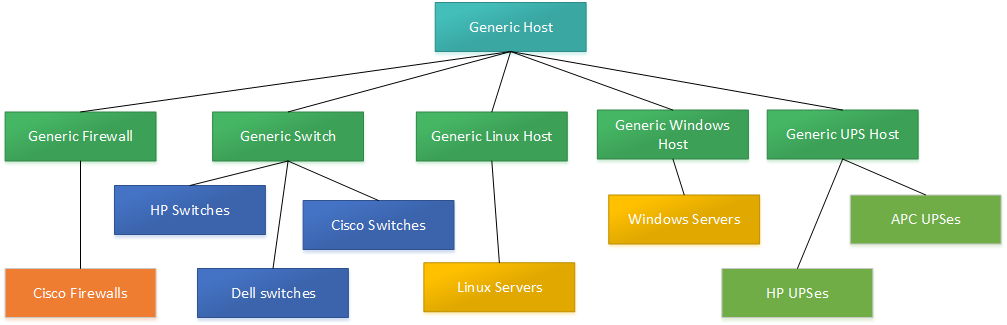
\includegraphics{img/host}
    \caption{Oversikt over host generic plassering}
    \label{hostfigur}
\end{figure}
\end{center}

I Figur \ref{hostgroupfigur} ser vi hvilke hostgroups de forskjellige hostene skal være medlem av.

\begin{center}
\begin{figure}
    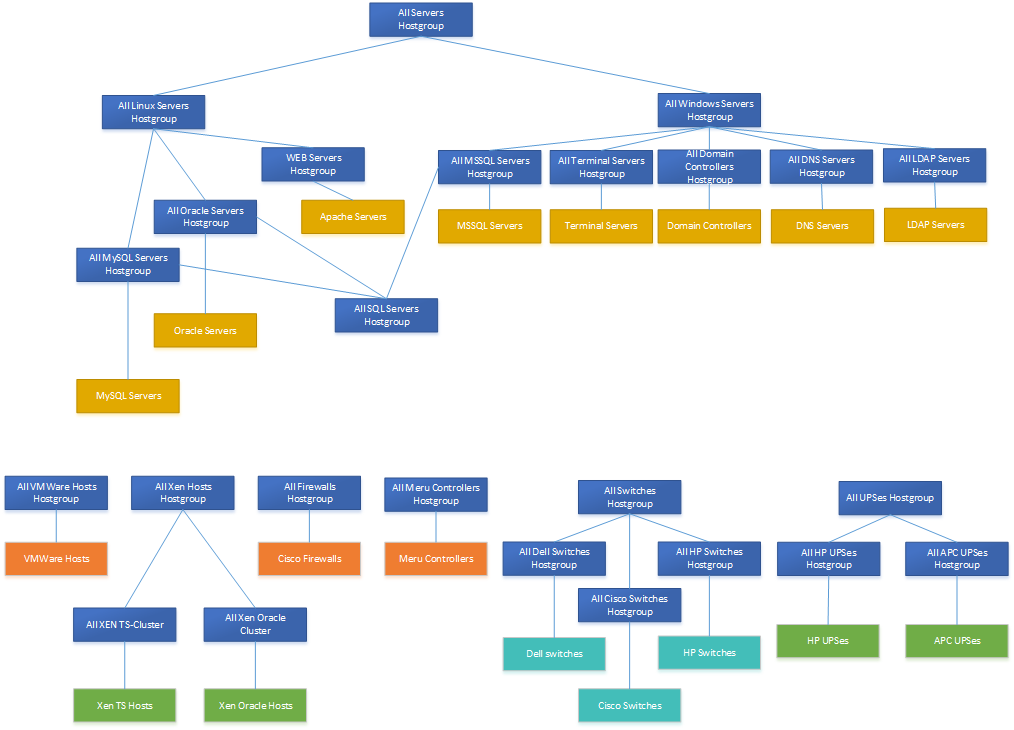
\includegraphics{img/hostgroups}
    \caption{Oversikt over hosts hostgroupplassering}
    \label{hostgroupfigur}
\end{figure}
\end{center}


\begin{itemize}
	\item Fremgang for nye enheter (host, hostgroup, templates osv)
        \item Arv og dependency
        \item Oversikt over services, commands og thresholds
        \item Acknowledgement av hosts og services
        \item Scheduled downtime
        \item Filhierarkiet
\end{itemize}
\subsection{Legge til mange host-objekter}
\begin{itemize}
	\item Et selvlaget script ref gen.bash brukes for å effektivt legge til mange hosts med Nils to reference his fancy smancy addhost-script med mulighet til å legge til hosts fra CSV-fil /ref{kildekode}
\end{itemize}
\subsection{Autentisering mot Active Directory} 
LDAP-autentisering brukes for å styre hvem som skal ha tilgang til web-grensesnittene, ved hjelp av grupper og brukere i Active Directory. Dette er støttet direkte i Icinga-web, men må konfigureres på andre måter for Icinga Classic. Det kan opprettes en sikkerhetsgruppe i AD som inkluderer medlemmene som skal få tilgang. Alle som er med i denne gruppen vil få tilgang til Icinga Web, der det også kan defineres hvilken informasjon hver bruker skal kunne se. 

Selve LDAP-binden gjøres via PHP-modulen “php-ldap”. Når en bruker logger inn sjekkes først AD, dersom brukeren ikke finnes der, vil Icinga-web prøve sin egen database over brukere. Hvis brukeren finnes her og passordet er riktig vil brukeren bli logget inn. Når brukeren har logget inn for første gang via AD, vil brukeren bli lagret i Icinga-Web databasen. Om brukeren endrer passord i Icinga-Web vil uansett AD først bli spurt før Icinga-Web spør om passordet er riktig i sin egen database

Icinga classic autentiserer mot AD gjennom modulene ldap og authnz\_ldap.

/etc/apache2/conf.d/

\begin{lstlisting}
        AuthName "Authentication"
        AuthType Basic
        AuthBasicProvider ldap
        AuthLDAPURL
"ldap://10.60.0.22:3268/dc=monkey,dc=local?samAccountName?sub?(objectClass=person)"
        AuthLDAPBindDN "flash@monkey.local"
        AuthLDAPBindPassword "Bachel0r"
        require ldap-group CN=icinga-login, OU=icinga, DC=monkey, DC=local
\end{lstlisting}

/usr/share/icinga-web/app/modules/AppKit/config/auth.xml

\begin{lstlisting}
  <ae:parameter name="ldap_allow_anonymous">false</ae:parameter>
            <ae:parameter name="ldap_dsn">ldap://10.60.0.22</ae:parameter>
            <ae:parameter name="ldap_start_tls">false</ae:parameter>
            <ae:parameter name="ldap_basedn">DC=monkey,DC=local</ae:parameter>
            <ae:parameter name="ldap_binddn">icingawebauth@monkey.local</ae:parameter>
            <ae:parameter name="ldap_bindpw"><![CDATA[Bachel0r]]></ae:parameter>
            <ae:parameter name="ldap_userattr">sAMAccountName</ae:parameter>
            <ae:parameter name="ldap_filter_user"><![CDATA[(&(sAMAccountName=__USERNAME__)(memberOf=CN=icinga-login,OU=icinga,DC=monkey,DC=local))]]></ae:parameter>
        </ae:parameter>
\end{lstlisting}

\subsection{Kontrakter og kontaktgrupper}

For å opprette en ny kontakt i Icinga meldes brukeren inn i gruppen icinga\_kontakter (se synkronisering). Den vil trenge å ha e-postadresse og telefonnummer satt.

Kontaktgrupper hentes fra OU-en icinga\_grupper der alle grupper hentes ut og opprettes i Icinga. For at en gruppe skal varsles må dette legges til på en service. For å slippe å sette opp kontakter for hver service kan en velge å sende med en parameter “gen\_service” for å generere en template som kan benyttes på tjenester som sorterer under hver av kontaktgruppene som blir opprettet.

Eksempel på generisk service som blir opprettet:

\begin{lstlisting}
define service {
    name network_services
    register 0
    use generic-service     
    notification_interval   30
    notification_period     24x7
    notification_options    w,c,r
    contact_groups          network_contact_group
}
\end{lstlisting}

Denne brukes på en cisco firewall: 

\begin{lstlisting}
define service {
        service_description Cisco Firewall CPU Load
        use network_services
        name cisco-firewall-cpu-load
        hostgroup_name all_firewalls
        check_command check_network_component!cpu-load
}
\end{lstlisting}
